\subsubsection{Measure}\label{sec:measure_view}
The measure tab allows for making controlled measurements with a simplified interface. These measurement can then be exported as clean, human readable reports while still being valid spectrum files. The interface is designed to be intuitive and this tab serves as the only interface for LuRaCs-Si, as described in the introduction. Buttons will indicate the order they should be pressed and the only submenus required are to connect detectors and to export the report. 

\begin{figure}[H]
    \centering
    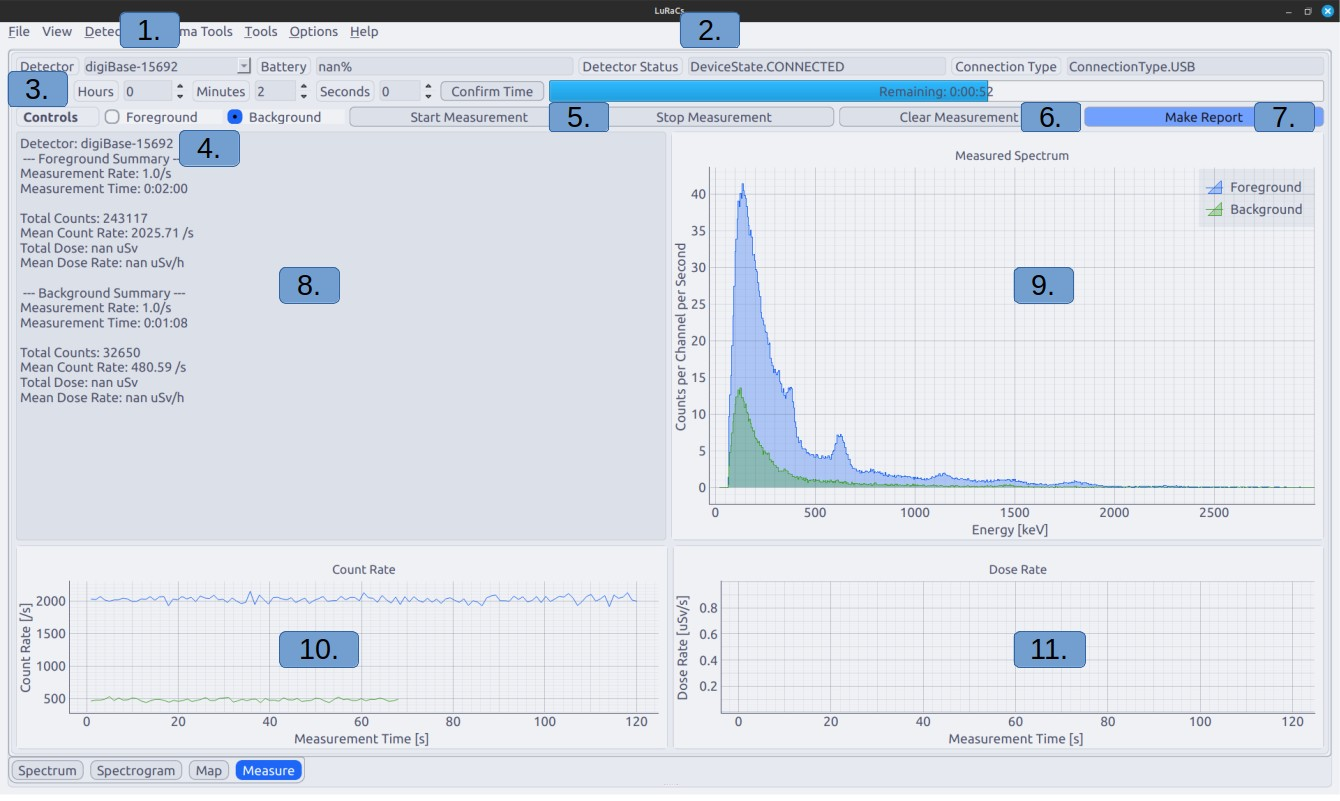
\includegraphics[width = .9\linewidth]{images/interface/measure_view.jpg}
    \caption{The measure view with an on going measurement using a 3"x3" NaI detector. The foreground spectrum is of an antique containing Ra-226 and the background is a regular office. The detector does not have a battery and does not output dose data, therefore these reading are \texttt{nan}.}
    \label{fig:measure_view}
    \begin{flushleft}
        \begin{enumerate}
            \item Selected detector. If the detector is changed all measurements are reset to avoid mixing measurements for different detectors. This is preceded by a question dialog so results are not lost by accident.
            \item Detector status bars, shows the same data as in the \textit{Detectors}-tab, see section \ref{sec:detectors}
            \item The measurement timer to determine the length of a measurement. The duration is set in the spinboxes and must be applied with \texttt{Confirm Time}, which while be marked upon changing a time value. The bar shows remaining time. The same time can be used for fore- and background without applying it again.
            \item Selects if the measurement is the fore- or background.
            \item \texttt{Start Measurement} and \texttt{Stop Measurement} do what they say. Each time an ongoing measurement is stopped the timestamp is logged and included in the report.
            \item Clears the measurement selected in (4.).
            \item Opens the Report Dialog for creating a report form the measurement, see \autoref{fig:report_form}.
            \item Main information window that displays summary information about the measurements.
            \item Count histogram of the fore- and background. Pulls the energy calibration form the spectrum in the \textit{Spectrum}-tab.
            \item Count Rate graph.
            \item Dose Rate graph, always in \unit{\micro\sievert\per\hour}
        \end{enumerate}
    \end{flushleft}
\end{figure}

\begin{figure}[H]
    \centering
    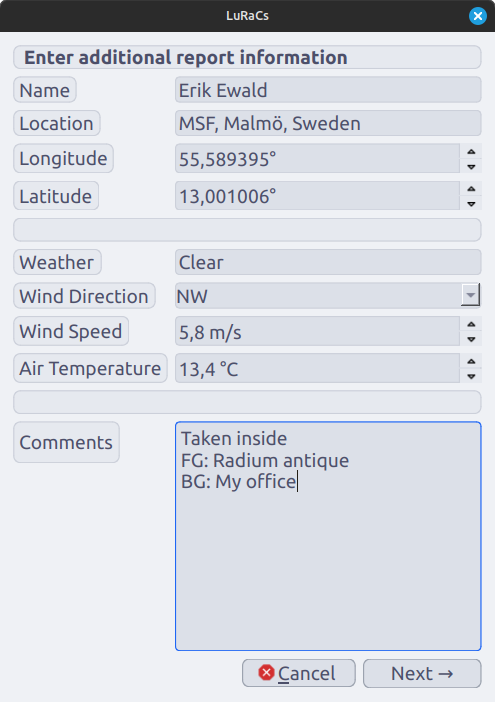
\includegraphics[width = .4\linewidth]{images/interface/report_form.png}
    \caption{Report Form opened by pressing (7.) in \autoref{fig:measure_view}.}
    \label{fig:report_form}
\end{figure}